\section{Processi di supporto}
In questa sezione verranno trattati i processi di supporto allo sviluppo del progetto.
\subsection{Comunicazioni}
\subsubsection{Comunicazioni interne}
L'apparato di comunicazioni interne ufficiali sarà gestito tramite una \textit{mailing list\ped{G}} basata su \textit{Google Groups}.\\
Il nome della \textit{mailing list} è Sirius esattamente come il nome del gruppo(\gruppo).\\ Vige l'obbligo di utilizzare la \textit{mailing list} solamente per le comunicazioni interne ufficiali, così da evitare intasamenti superflui che graverebbero sul lavoro di verbalizzazione delle comunicazioni di rilevo, in quanto renderebbero più complessa ed inutilmente lunga l'estrazione delle informazioni utili. Tuttavia è preferibile che la comunicazione tra i vari componenti del team avvenga principalmente durante gli incontri che si terranno in un luogo fisico comune (sezione 2.2, Riunioni interne).\\
Al fine di facilitare anche le comunicazioni informali, sono stati adottati due strumenti di \textit{instant messaging\ped{G}} e videoconferenza quali Skype e Google Plus ed un strumento di \textit{web storage} per lo scambio di dati ufficiosi (sezione 8.1, Gestione condivisione file).

\subsubsection{Riunioni interne}
Le riunioni del gruppo \gruppo{} avranno una frequenza almeno settimanale. Il giorno della settimana, il luogo e l'ora in cui riunirsi ufficialmente sarà deciso dal \textit{Responsabile di Progetto} su consultazione degli altri membri del team e sarà comunicato tramite il gruppo \textit{Google Groups} Sirius. Chiunque non abbia la possibilità di essere presente fisicamente nel luogo della riunione, dovrà possibilmente restare in contatto con il nucleo dei membri mediante videoconferenza.\\
Qualunque membro del team può richiedere al \textit{Responsabile di Progetto} di indire una riunione allegandone l'argomento di discussione ed una sua breve descrizione, a seguito della comunicazione il \textit{Responsabile di Progetto} deciderà se indire la suddetta riunione generale, cioè con obbligatoria presenza di tutti i membri del gruppo. Qualsiasi riunione surplus a quella settimanale deve essere indetta con almeno 2 giorni di anticipo, in modo da verificare la disponibilità del gruppo.\\
Se dovessero essere necessarie riunioni che non richiedono la presenza del gruppo nella sua totalità, ogni membro potrà presentare la richiesta di ritrovo tramite l'apposita \textit{mailing list} (sezione 2.1, Comunicazioni interne), richiedendo la disponibilità degli specifici membri del team che riterrà necessari, questo poiché è auspicabile che alcune figure come ad esempio \textit{Progettista} ed \textit{Analista} collaborino tra di loro frequentemente.\\
Le riunioni che non coinvolgono interamente il team non necessitano dell'approvazione del \textit{Responsabile di Progetto} in modo da ridurre il suo carico di lavoro, nonostante questo le decisioni effettuate durante queste discussioni inter-membri dovranno comunque essere verbalizzate.

\subsubsection{Comunicazioni Esterne}
Per le comunicazioni esterne di ogni tipo è stato creato in indirizzo \textit{e-mail} del team:
\begin{center}
\href{swesirius@gmail.com}{swesirius@gmail.com}
\end{center}

Il \textit{Responsabile di Progetto} rappresenta il team stesso, sarà quindi incaricato di mantenere i contatti con proponente, committente, ed eventuali altre figure non facenti parte del nucleo del \textit{team}, tramite questo indirizzo \textit{e-mail}, inoltre sarà sempre parte del suo compito aggiornare i membri del gruppo stesso riguardo le corrispondenze pervenute attenendosi alle istruzioni della sezione 2.1, Comunicazioni interne.

\subsubsection{Incontri esterni}
Il \textit{Responsabile di Progetto} ha inoltre l'onere di organizzare eventuali incontri esterni (per chiarificazioni o quant'altro) con \textit{Proponente} o \textit{Committente/i}. Ogni membro del gruppo può richiedere un incontro esterno al \textit{Responsabile di Progetto}, presentando una motivazione valida.
Infine, il \textit{Responsabile di Progetto} dopo aver valutato personalmente la proposta, dovrà presentarla al gruppo (con allegata la motivazione ed il nome di chi l'ha richiesta) quindi, per l'approvazione definitiva di quest'ultima, almeno due membri escluso l'artefice dovranno dare ulteriore conferma e disponibilità, in caso contrario la proposta sarà bocciata.
\subsubsection{Strumenti per le comunicazioni}
Oltre agli strumenti precedentemente citati quali: Skype, Google Hangout, mailing list Google, per gestire efficientemente la condivisione dei file intra-gruppo è stato scelto l'utilizzo di: Google Drive, un servizio \textit{web} di \textit{storage} e sincronizzazione \textit{online} che dovrebbe facilitare la condivisione e fornire una base d'appoggio secondaria ed informale per alcuni file che non necessitano versionamento.
L'utilizzo di \textit{Google Drive} e' limitato ai documenti che:
\begin{itemize}
\item Non necessitano di versionamento;
\item Necessitano di essere acceduti velocemente tramite \textit{web};
\end{itemize}
\subsection{Documentazione}
\subsubsection{Template}
Ogni documento dovrà essere generato includendo il \textit{template} \LaTeX presente nella cartella "Modello".
Questo modello è stato creato prima dell'inizio della redazione di ogni altro documento del team \gruppo{}, la sua modifica può avvenire solo presentando all'\textit{Amministratore} una richiesta formale, allegandone la motivazione ed il tipo di modifica richiesta. Se l'\textit{Amministratore} riterrà opportuno effettuare il cambiamento, prima di apportare la modifica dovrà avvertire l'intero team al fine di evitare disguidi.

\subsubsection{Classificazione documenti}
\paragraph{Documenti formali}
Sono catalogati come formali tutti i documenti approvati dal \textit{Responsabile di Progetto}, ovvero i documenti ritenuti pronti per essere visionati dal committente. Tali documenti, prima di raggiungere l'approvazione dovranno aver superato con successo la procedura di verifica e validazione riportata nel \textit{Piano di Qualifica}.
\paragraph{Documenti informali}
Tutti i documenti che non sono stati approvati dal \textit{Responsabile di Progetto} sono da ritenersi informali, e di utilizzo esclusivamente interno. Tutti i documenti non versionati sono da ritenersi non ufficiali.

\subsubsection{Versionamento documenti}
Il versionamento di tutta la documentazione del gruppo \gruppo{} è stato organizzato secondo le seguenti convenzioni:
\begin{itemize}
\item Il numero di versionamento deve essere nella forma:

\begin{center}
\textbf{X}, \textbf{Y}, \textbf{Z}
\end{center}

con \textbf{X}, \textbf{Y}, \textbf{Z} numeri interi non negativi;
\item Tutti gli elementi devono salire di una sola unità alla volta.
\end{itemize}

Di seguito vengono inoltre riportati i significati che possono assumere le variazioni della versione del documento:
\begin{itemize}
\item La \textbf{X} rappresenta il numero di uscite formali del documento, ogni qual volta un documento verrà pubblicato il valore della cifra \textbf{Y} e della cifra \textbf{Z} verrà azzerato. Riportando quanto detto più precisamente:
\begin{enumerate}
\item X assumerà il valore: 1, alla \textbf{revisione dei requisiti};
\item X assumerà il valore: 2, alla \textbf{revisione di progettazione};
\item X assumerà il valore: 3, alla \textbf{revisione di qualifica};
\item X assumerà il valore: 4, alla \textbf{revisione di accettazione}.
\end{enumerate}
\item La \textbf{Y} rappresenta il numero di \textit{push} effettuati sul \textit{branch\ped{G}} \textit{master} in \textit{GitHub} (sezione 8.2.1, GitHub), ossia il numero di volte in cui sono state compiute importanti modifiche al documento. Ogni qual volta aumenterà l'indice \textbf{Y} si azzererà l'indice \textbf{Z}.
\item La \textbf{Z} rappresenta il numero di modifiche minori apportate al documento durante il suo sviluppo.
Aumenta al termine di ogni sessione di lavoro sul documento.
\end{itemize}

Ogni documento formale riporterà un diario delle modifiche contenente le trasformazioni più rilevanti che ha attraversato sotto forma tabellare.

\subsubsection{Struttura Documentazione}
\paragraph{Header}
Ogni pagina esclusa la prima presenta un \textit{header} raffigurante il logo del gruppo sulla sinistra, mentre sulla destra il nome del team ed il nome del progetto.
\paragraph{Footer}
Ogni pagina esclusa la prima presenta un \textit{footer} riportante il nome del documento corredato della versione sulla sinistra, mentre sulla destra il numero della pagina.
Per il numero di pagina delle prime quattro facciate saranno utilizzati i numeri romani, a seguire invece verranno utilizzati i numeri occidentali.
\paragraph{Prima pagina}
La prima pagina di ogni documento conterrà:
\begin{itemize}
\item Il logo del \textit{team}, riportante la scritta \gruppo;
\item Il titolo del progetto;
\item Il nome del documento e la sua versione;
\item Il nome del corso;
\item L'anno di sviluppo del progetto;
\end{itemize}

\paragraph{Seconda pagina}
La seconda pagina di ogni documento conterrà:
\begin{itemize}
\item  Informazioni sul documento come segue:
\begin{itemize}
\item Titolo del documento;
\item Data di creazione;
\item Versione attuale;
\item Utilizzo, che specifica se il documento è per utilizzo interno o esterno;
\item Nome file;
\item Redazione;
\item Revisione;
\item Approvazione;
\item Distribuito da, a cui seguirà il nome del gruppo.
\end{itemize}
\item Un sommario riportante una breve descrizione;
\end{itemize}

\paragraph{Terza pagina}
La terza pagina di ogni documento conterrà:
\begin{itemize}
\item Un diario delle modifiche apportate al documento, dall'inizio fino alla versione corrente.
\end{itemize}

\paragraph{Quarta pagina}
La quarta pagina di ogni documento ne riporterà l'indice, è possibile che l'indice si estenda per più di una singola pagina. 

\subsubsection{Norme tipografiche}
\paragraph{Generali}
\begin{itemize}
\item Ogni documento deve essere in lingua italiana, altre lingue possono essere utilizzate per riferirsi a termini tecnici informatici o in situazioni che lo richiedono strettamente;

\item Ogni documento deve essere grammaticalmente, sintatticamente e semanticamente corretto, cercando di essere meno verboso possibile;

\item Utilizzare il più possibile elenchi puntati invece di lunghe frasi.

\end{itemize}
\paragraph{Punteggiatura}
\begin{itemize}
\item Non si usa mai un punto alla fine di un titolo: di capitolo, di paragrafo, di sotto-paragrafo;

\item Ogni elemento di un elenco puntato termina con un punto e virgola, se è l'ultimo elemento con un punto;

\item Prima di ogni segno di punteggiatura non va mai messo uno spazio bianco, dopo invece lo spazio bianco va messo sempre;


\item Il testo racchiuso tra parentesi non deve aprirsi o chiudersi con un carattere di spaziatura ne terminare con un carattere di punteggiatura.

\end{itemize}
\paragraph{Ortografia}

\begin{itemize}

\item Le lettere maiuscole vanno poste solo all'inizio di ogni elemento di un elenco puntato e dove lo prevede l'ortografia italiana (all'inizio di un periodo o dopo un segno di punteggiatura forte, cioè dopo il punto fermo, i puntini di sospensione, il punto esclamativo ed il punto interrogativo). È inoltre utilizzata l'iniziale maiuscola nel nome del team, del progetto, dei documenti, dei ruoli di progetto.


\end{itemize}

\paragraph{Stile}
\begin{itemize}
\item Se si devono elencare delle di istruzioni in serie o una divisione in paragrafi e sotto-paragrafi è necessario utilizzare un elenco numerato, altrimenti è preferibile un elenco puntato;

\item Il primo livello di profondità degli elenchi puntati è contrassegnato da un pallino nero pieno, il secondo da un trattino, il terzo da un asterisco;

\item Le date dovranno essere espresse nella forma \textbf{aaaa-mm-gg} secondo lo standard  \ped{G}\textbf{ISO G 8601:2004};

\item Gli orari dovranno essere espressi nella forma \textbf{hh:mm} secondo lo standard \textbf{ISO G 8601:2004};

\item \textbf{URL} ed indirizzi mail dovrano essere preceduto dal comando \LaTeX \verb+ \+url;

\item Ogni prima (e possibilmente anche successiva) occorrenza di una parola presente sul \textit{Glossario} sarà seguita da pedice \ped{G}.

\item Stile di testo:

\begin{itemize}

\item Il corsivo deve essere utilizzato obbligatoriamente nelle citazioni, per il nome delle figure di rilievo (es. \textit{committente}, \textit{Responsabile di Progetto}) e per il nome dei documenti (es. \textit{Analisi dei requisiti}), mentre a discrezione del redattore per termini stranieri in modo da evidenziarli;

\item il grassetto deve essere utilizzato per evidenziare (se si reputa necessario) le parole chiave ed i passaggi particolarmente rilevanti.

\end{itemize}

\end{itemize}
\subsubsection{Calcolo indice di Gulpease}
In ogni documento redatto il verificatore dovrà calcolare l'indice di Gulpease, ossia il valore di leggibilità del documento.
Per raggiungere il seguente scopo è disponibile uno \textit{script online}, reperibile al sito:\\
\\
\href{http://xoomer.virgilio.it/roberto-ricci/variabilialeatorie/esperimenti/leggibilita.htm}{http://www.xoomer.virgilio.it/roberto-ricci/variabilialeatorie/esperimenti/leggibilita.htm}
\\ \\
Questo \textit{script} già esistente è stato verificato prima di essere adottato, in modo da scongiurare il rischio di incompatibilità tra i documenti redatti e la forma che doveva avere l'input per lo \textit{script}.
Se l'indice risultante di un documento si troverà in un range compreso tra lo 0 ed il 40, sarà necessario ricercare nel testo frasi troppo lunghe e complesse per reimpostarle.


\subsubsection{Glossario}
Durante la stesura di un documento, ogni qual volta il redattore riterrà necessario chiarire il significato di un termine utilizzato sarà tenuto ad aggiungerlo nel \textit{glossario}.\\
Il \textit{glossario} sarà strutturato seguendo questo schema:
\begin{itemize}
\item Nel file \LaTeX ogni parola sarà contenuta nel \textbf{tag}: "elemento";
\item A seguire, andando a capo-riga, sarà riportata la descrizione del termine.
\end{itemize}
Il \textit{glossario} sarà inoltre suddiviso in due sezioni:
\begin{itemize}
\item Termini;
\item Acronimi.
\end{itemize}
Termini ed acronimi dovranno essere necessariamente elencati in ordine alfabetico, la definizione dovrà essere breve ed esplicativa, inoltre sempre la definizione non potrà iniziare con una \textbf{E accentata}.
\subsubsection{Strumenti per la documentazione}
\paragraph{LaTeX}
Per la stesura dei documenti il team \gruppo{} ha deciso di adottare il linguaggio di markup\ped{G} \LaTeX la scelta è stata effettuata prevalentemente per le seguenti ragioni:
\begin{itemize}
\item Facilità di separazione tra contenuto
e formattazione;
\item Possibilità di definire macro ed incorporare scripts;
\item Software open source;
\item Grande quantità di pacchetti disponibili, possibilità quindi di implementare semplicemente le funzionalità comuni.
\end{itemize}
Gli altri software valutati (Open office, Microsoft Office, Google Docs) non erano in grado di fornire il più delle sopracitate funzionalità, di conseguenza sono stati scartati. Inoltre come editor è consigliato ma non obbligato l'uso di TeXstudio.

\paragraph{Macro}
Al fine di velocizzare il lavoro di stesura documenti, il team \gruppo{} ha deciso di creare delle apposite macro, qui vengono riportate le principali assieme ad una breve spiegazione delle loro funzionalità:
\begin{itemize}
\item \verb+\+gruppo riporta il nome del team \gruppo;
\item \verb+\+progetto riporta il nome del progetto: \progetto;
\item \verb+\+lastversion+sigla-del-documento riporta il nome del documento che appare in sigla (NDP, AR, etc..) aggiornato alla versione più recente.

\end{itemize}
\paragraph{Scripts}
Al fine di implementare una funzionalità quale l'inserimento automatico dei pedici in tutte le parole dei documenti formali che comparivano anche nel glossario, è stato creato uno script apposito in Pyton\ped{G}. Tale script può essere essere eseguito solamente con una versione di Pyton non superiore alla 2.7.6.
Per il corretto funzionamento dello script il glossario è stato organizzato tramite tag \LaTeX elemento{"parola del glossario"}, la definizione è riportata a capo-riga rispetto alla suddetta parola. 

\paragraph{Correttezza}
\paragraph{Correttezza ortografica}
Per evitare di compiere errori di tipo ortografico devono essere adottate due precauzioni:
\begin{itemize}
\item Verifica delle parole durante la stesura stessa del documento tramite lo spell checker\ped{G} di TeXstudio;
\item Verifica finale tramite lo spell checker Aspell.
\end{itemize}
Lo spell checker di TeXstudio è una sua feature\ped{G} molto utile che sfrutta dizionari Open Office per sottolineare eventuali parole scorrette, dizionari sufficientemente completi che assicurano quindi un grado piuttosto elevato di correttezza già durante la stesura del testo. \\
Al fine poi di assicurarsi il massimo grado possibile di correttezza viene effettuata una verifica ulteriore tramite il software open source GNU Aspell
(\href{http://www.aspell.net/}{www.aspell.net}).
 
\paragraph{Lista controllo errori}
Il team ha stilato una lista di controllo al fine di riassumere gli errori più ricorrenti in ogni documento, i suddetti saranno catalogati e descritti nella seguente sezione.
\paragraph{Errori stilistici e di punteggiatura}
I principali errori rilevati sono i seguenti:
\begin{itemize}
\item Le figure di rilievo non vengono scritte in corsivo;
\item Negli elenchi puntati la prima parola non compare con la prima lettera maiuscola;
\item Negli elenchi puntati alcuni elementi centrali non terminano con un punto e virgola ma con un punto fermo;
\item Alcune date vengono erroneamente scritte senza seguire lo standard \textbf{ISO G 8601:2004};
\item La parola LaTeX compare senza l'utilizzo del comando \verb+\+LaTeX (\LaTeX).
\end{itemize}
\paragraph{Errori ortografici e di sintassi}
\begin{itemize}
\item La è accentata compare (erroneamente) come una e apostrofata;
\item Utilizzando le seguenti macro \verb+\+gruppo e \verb+\+progetto, le quali scrivono testualmente e rispettivamente il nome del team ed il nome del capitolato, non compaiono separate dalla parola successiva, anche se la spaziatura è presente;
\item Non viene utilizzata (erroneamente) la terza persona per la stesura dei documenti.
\end{itemize}
\paragraph{UML}
Per la modellazione dei diagrammi User Case (UC\ped{G}) sono stati presi in considerazione tre editor: Dia, Microsoft Visio, Astah. Infine il team ha optato per adottare Astah come strumento definitivo in quanto si tratta di un software open source, con supporto di Unified Modeling Language (UML\ped{G}) 2.x  e secondo l'analisi del team dotato di un interfaccia più responsiva ed intuitiva degli altri software.

Per lo sviluppo dei diagrammi di sequenza, dopo aver effettuato i test necessari, è stato permesso l'utilizzo del software \textit{VisualParadigm}, questa modifica è stata attuata dopo aver verificato che il software \textit{Astah} forniva un iterfaccia di creazione per diagrammi di sequenza poco intuitiva e difficoltosa da utilizzare. \textit{VisualParadigm} è adeguato per lo sviluppo di diagrammi UML 2.x.

\subsection{Gestione configurazione}
La gestione di configurazione deve comprendere tutte le attività necessarie a rendere affidabile l'evoluzione del progetto,
tenendo traccia delle sue versioni.
\subsubsection{Strumento di versionamento}
Di pressoché fondamentale importanza è stata la definizione di un ambiente ordinato in cui organizzare e mantenere tutti i \textit{file} che attraversano il ciclo di vita, per questa ragione è stato scelto di avvalersi di un \textit{repository}. 

\paragraph{GitHub}
Come sistema di controllo di versione è stato adottato il software \textit{GitHub\ped{G}}, i pregi di questo strumento vengono qui di seguito riportati:
\begin{itemize}
\item Molto reattivo;
\item Design semplice; 
\item \textit{Software} gratuito.
\end{itemize}

\paragraph{Struttura repository}
L'indirizzo di \textbf{root\ped{G}} del \textit{repository} contenente tutta la documentazione è:
\begin{center}
\href{https://github.com/Dquaglio/Sirius}{https://github.com/Dquaglio/Sirius}
\end{center}

Ogni documento presente sarà contenuto in una sotto cartella del \textit{master branch\ped{G}} nominata come il nome del documento stesso.
All'interno della cartella potranno essere contenuti solamente \textit{file.tex}, per la visualizzazione del relativo \textit{pdf\ped{G}} sarà necessario scaricarli e compilarli, assicurandosi di avere l'ultima versione del modello disponibile.
\begin{center}
\textbf{modello.git}: \href{https://github.com/Dquaglio/Sirius/tree/master/modello.git}{https://github.com/Dquaglio/Sirius/tree/master/modello.git}
\end{center}

conterrà il \textit{template} \LaTeX, le \textit{macro} e gli script aggiornati all'ultima versione disponibile.
\\
\\
Il \textit{master branch} è stato quindi suddiviso seguendo questa struttura:
\begin{figure}
\centering
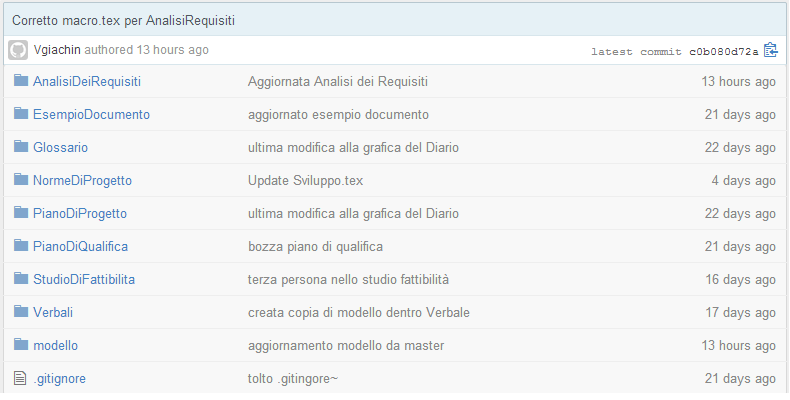
\includegraphics[width= %
\linewidth]{immaginiNDP/repository}
\caption[]{Struttura master branch.}
\label{fig:repository}
\end{figure}
A scopo puramente dimostrativo è stato creato l'esempio di un documento formale del gruppo \gruppo, contenuto nella cartella: "EsempioDocumento", questa scelta è stata fatta per illustrare la struttura generale che deve preservare qualsiasi documento (sezione 5.4, Struttura documentazione).
Per sfruttare il parallelismo nello sviluppo di uno stesso documento sono stati creati appositamente dei  \textit{branch} denominati con il nome dei membri del gruppo, i documenti  \textit{baseline\ped{G}} invece saranno contenuti solamente nel \textit{master branch}. Il \textit{merge\ped{G}} con il ramo \textit{master} avviene quindi solamente dopo la terminazione dell'attività di verifica di un documento.

\subsection{Verifica}
\subsubsection{Metriche}
I dati rilevati durante l'attività di verifica devono essere analizzati tramite precise metriche.
Con questo termine si intende l'insieme di parametri misurabili su un processo. Qualora le metriche definite in questo documento siano approssimative e/o ambigue, queste dovranno essere ridefinite in modo specifico e seguiranno in modo incrementale il ciclo di vita del prodotto. Di seguito sono riportate le metriche adottate dal team \textit{Sirius}; gli obbiettivi qualitativi che invece definiscono il grado di accettazione/ottimalità verranno riportati nel \PianoDiQualifica.
\paragraph{Metriche per i processi}
Le metriche dei processi ne stabiliscono la qualità, definita come connubio tra \textit{capability}\ped{G}, \textit{maturity}\ped{G} e i miglioramenti. Queste caratteristiche di qualità si possono individuare in tre classi di misure di processo:
\begin{itemize}
\item \textbf{Tempo}: il tempo richiesto per il completamento di un particolare processo;
\item \textbf{Risorse}: le risorse richieste per un particolare processo, in genere vengono definite risorse-uomo, per le risorse software si fa riferimento a \infoNDP;
\item \textbf{Occorrenze}: il numero di volte che capita un particolare evento, che può essere il numero di difetti scoperti durante l'attività di verifica.
\end{itemize}
Per rilevare questi dati \gruppo ~ha deciso di utilizzare, indici che valutano i tempi e i costi del processo. La scelta di queste metriche è dettata anche dal loro possibile utilizzo durante lo svolgimento del processo, per capire in modo semplice se lo stato del processo è conforme a quanto pianificato, mantenendo quindi il processo in controllo. In \infoPDP ~viene specificato come sono stati pianificati questi indici nello stato di avanzamento.
\paragraph{(SV) Schedule Variance}
Indica se si è in linea, in anticipo o in ritardo rispetto alla pianificazione temporale delle attività citata in \infoPDP.
È un indicatore di efficacia temporale e per questo \gruppo ha deciso di esprimerlo in ore.
Se SV $>$ 0 significa che il gruppo di lavoro sta producendo con maggior velocità rispetto a quanto pianificato, viceversa se negativo.\\

\paragraph{(BV) Budget Variance}
Indica se allo stato attuale si è speso più o meno rispetto a quanto pianificato.
È un indicatore che ha valore contabile e finanziario per questo è espresso in euro.
Se BV $>$ 0 significa che l’attuazione del progetto sta consumando il proprio budget con minor velocità rispetto a quanto pianificato, viceversa se negativo.

\paragraph{Metriche per i documenti}
Come metrica per la verifica dei documenti \gruppo ha deciso di utilizzare l’indice di leggibilità.
Vi sono a disposizione molti indici di leggibilità, ma i più importanti sono per la lingua inglese. Si è deciso quindi di adottare un indice di leggibilità per la lingua italiana.
L’indice \textit{Gulpease} è un indice di leggibilità di un testo tarato sulla lingua italiana. Rispetto ad altri indici, esso ha il vantaggio di utilizzare la lunghezza delle parole in lettere anziché in sillabe, semplificandone il calcolo automatico. Permette di misurare la complessità dello stile di scrittura di un documento.
L’indice viene calcolato utilizzando la formula citata nelle \infoNDP~.
I risultati sono compresi tra 0 e 100, dove il valore 100 indica la leggibilità più alta e 0 la leggibilità più bassa. In generale risulta che testi con un indice:
\begin{itemize}
\item Inferiore a 80 sono difficili da leggere per chi ha la licenza elementare;
\item Inferiore a 60 sono difficili da leggere per chi ha la licenza media;
\item Inferiore a 40 sono difficili da leggere per chi ha un diploma superiore.
\end{itemize}

\paragraph{Metriche per il software}
Al fine di perseguire gli obiettivi qualitativi dichiarati nel \PianoDiQualifica{} è necessario definire delle metriche, queste metriche hanno quindi l'obbiettivo di rendere quantificabile il lavoro svolto. Questa sezione, però, è da intendersi come modificabile nell'arco dello svolgimento del progetto.
\paragraph{Complessità ciclomatica}
Pensata da T.J. McCabe è utilizzata per misurare la complessità per funzioni, moduli, metodi o classi di un programma. Misura direttamente il numero di cammini linearmente indipendenti attraverso il grafo di controllo di flusso.
Alti valori di complessità ciclomatica indicano una ridotta manutenibilità del codice. Al contrario, valori bassi potrebbero determinare una scarsa efficienza dei metodi. Questo parametro è inoltre un indice del carico di lavoro richiesto dal \textit{testing}. Indicativamente un modulo con complessità ciclomatica più bassa richiede meno test di uno con complessità più elevata.\\
Il valore 10 come massimo di complessità ciclomatica fu raccomandato da T.J.McCabe, l'inventore di tale metrica.
\paragraph{Numero livelli di annidamento}
Rappresenta il numero di livelli di annidamento, quindi l'inserimento di una struttura di controllo all'interno di un'altra. Un elevato valore comporta un'alta complessità e un basso livello di astrazione del codice.\\

\paragraph{Attributi per classe}
Un elevato numero di attributi per classe può rappresentare la necessità di suddividere la classe in più classi, possibilmente utilizzando la tecnica dell'incapsulamento, e può inoltre rappresentare un possibile errore di progettazione.\\

\paragraph{Numero di parametri per metodo}
Un elevato numero di parametri potrebbe richiedere di ridurre le funzionalità del metodo o provvedere ad una nuova progettazione dello stesso.\\

\paragraph{Linee di codice per linee di commento}
Indica il rapporto tra linee di codice e linee di commento: questo parametro è fondamentale per valutare la manutenibilità del codice prodotto, nonché del possibile riuso.\\

\paragraph{Accoppiamento}
\begin{itemize}
\item \textbf{Accoppiamento afferente:} indica il numero di classi esterne al package\ped{G} che dipendono da classi interne ad esso. Un alto valore indica che è presente un alto grado di dipendenza del resto del software dal package. Questo non indica necessariamente una progettazione errata o di bassa qualità, ma possono rappresentare una criticità del package, che quindi perderebbe di robustezza. Al contrario un valore troppo basso potrebbe segnalare che il package analizzato fornisce poche funzionalità e quindi potrebbe risultare scarsamente utile.
\textbf{Parametri utilizzati:}
I valori di range di tale indice verranno definiti durante la progettazione di dettaglio.
\item \textbf{Accoppiamento efferente:} indica il numero di classi interne al package che dipendono da classi esterne ad esso. Mantenendo un basso valore di questo indice, è possibile mantenere il package in grado di garantire funzionalità di base indipendentemente dal resto del sistema.
\end{itemize}
\paragraph{Copertura del codice}
Indica la percentuale di istruzione che vengono eseguite durante i test. Maggiore è la percentuale e più probabilità si hanno di rilevare minori errori nei prodotto. Tale valore può essere abbassato tramite l'utilizzo di metodi molto semplici che non richiedono test.\\
\subsubsection{Procedure di verifica}
\paragraph{Tecniche di analisi statica}
L'analisi statica è una tecnica di analisi applicabile sia alla documentazione che al codice e permette di effettuare la verifica di quanto prodotto individuando errori ed anomalie. Essa può essere svolta in due modi diversi ma complementari tra di loro in quanto per utilizzare \textit{inspection} bisogna prima aver effettuato \textit{walkthrough}
\subparagraph{Inspection}
Questa tecnica, di analisi statica, consiste nella verifica di sezioni ben definite di un documento o del codice. Questo tipo di controlli per i documenti sono usualmente definiti tramite una lista di controllo (checklist) redatta anticipatamente rispetto all'attività di verifica da intraprendere. Per la verifica dei documenti, la lista di controllo è stata elaborata a seguito di analisi eseguite tramite \textit{walkthrough}, ed evidenziando gli errori più ricorrenti riscontrati. \textit{Inspection} è una strategia rapida in quanto permette l'analisi di alcuni parti ritenute critiche nella checklist senza bisogno di una lettura integrale di documento o di tutto il codice in oggetto.
\subparagraph{Walkthrough}
\textit{Walkthrough} è una tecnica di analisi statica che consiste nella lettura critica a largo raggio di tutto il documento. In questa tipologia di analisi il \textit{Verificatore} utilizza molto tempo per la lettura e correzione del documento o codice. Questa tecnica viene di solito utilizzata nella prima parte dello sviluppo di progetti in quanto, la poca esperienza del \textit{Verificatore} non permette un'altro tipo di verifica. Al termine di questo primo set di analisi \textit{walkthrough} viene usualmente definita una lista di controllo che permetta di ricercare in primo luogo gli errori più ricorrenti, e maggiormente riscontrati. \textit{Walkthrough} è un'attività onerosa e collaborativa che richiede l'intervento di più persone per essere efficiente ed efficace
\paragraph{Tecniche di analisi dinamica}
L'analisi dinamica si applica solamente al prodotto software e consiste nell'esecuzione del codice mediante l'uso di test predisposti per verificarne il funzionamento o rilevare possibili difetti di implementazione eseguendo tutto o solo una parte del codice.
La \textbf{ripetibilità} del test è una caratteristica fondamentale per questo tipo di test, in quanto dichiara che il codice con un certo \textit{input} produce sempre lo stesso \textit{output} su uno specifico ambiente. In questo modo si è in grado di riscontrare problemi e verificare la correttezza del prodotto.
Per questo \gruppo ~ha deciso di definire a priori le seguenti caratteristiche:
\begin{itemize}
\item \textbf{Ambiente}: sistema \textit{hardware} e quello \textit{software} sui quali è stato pianificato l'utilizzo del prodotto, di essi si deve definire uno stato iniziale dal quale poter iniziare ad eseguire i test;
\item \textbf{Specifica di \textit{input}}: definire quali sono gli \textit{input} e quali devono essere gli \textit{output} attesi;
\item \textbf{Procedure}: definire quali devono essere i test ed in che ordine devono essere analizzati i risultati ottenuti.
\end{itemize}
Di seguito sono definiti cinque diversi tipi di test.
\subparagraph{Test di unità} 
Per test di unità si intende la verifica di ogni singola unità di prodotto software tramite l'utilizzo di stub\ped{G}, driver\ped{G} e logger\ped{G}. Per unità si intende la più piccola porzione di codice che è utile verificare singolarmente e che viene prodotta da un unico programmatore. Tramite questo tipo di test si vogliono testare i vari le unità per rilevare errori di implementazione da parte dei programmatori.
\subparagraph{Test di integrazione}
I test di integrazione prevedono la verifica dei componenti del sistema che vengono aggiunti incrementando il prodotto di origine e si prefigge quindi di analizzare la combinazione di due o più unità software che hanno quindi superato i test di unità. Questa tecnica di verifica serve ad individuare errori residui nella programmazione dei singoli moduli: come modifiche delle interfacce e comportamenti inaspettati di componenti software di parti terze e che pregiudicherebbero la validità del prodotto. Per effettuare tali test può essere necessario l'aggiunta di componenti software fittizie e non ancora implementate al fine di non pregiudicare negativamente l'esito dell'analisi.
\subparagraph{Test di sistema}
Consiste nella validazione del sistema attraverso la verifica della copertura di tutti i requisiti obbligatori individuati in \infoAR, e tracciati  grazie allo strumento messo a punto da \gruppo;
\subparagraph{Test di regressione}
I test di regressione vengono eseguiti quando si apportano delle modifiche a parte del software e questi consistono nella riesecuzione dei test riguardanti le i componenti che hanno subito modifiche e che precedentemente non erano soggetti ad errori.
Tale operazione viene aiutata dal tracciamento, che permette di individuare e ripetere facilmente i test di unità, integrazione ed eventualmente di sistema che sono stati potenzialmente influenzati dalle modifiche.
\subparagraph{Test di accettazione}
Si tratta del collaudo del prodotto software sotto il controllo del proponente. Se il collaudo viene superato in modo positivo, il sistema viene rilasciato e la commessa si conclude.
\subsubsection{Strumenti per la verifica}
\paragraph{Strumenti per testing}
Per quanto concerne gli strumenti utilizzati per la stesura dei test, i test lato server si baseranno sull'ausiglio di:
\begin{itemize}
\item \textit{Eclipse metrics}, che fornisce un tool di testing per codice \textit{Java} in grado di evidenziare la copertura fornita dai test;
\item \textit{JUnit}, framework per effettuare test \textit{Java};
\item \textit{Mockito}.
\end{itemize}
mentre lo sviluppo di test lato client si baserà su:
\begin{itemize}
\item \textit{Jasmine} un framework per effettuare test \textit{JavaScript}.
\end{itemize}
Per quanto concerne la copertura del codice \textit{JavaScript} si utilizzerà \textit{Istanbul}.